\documentclass[sigconf]{acmart}

\fancyhf{} %]{Anonymous submission \#99ACM CCS 2017} % TODO: replace 9999 with your paper number
\fancyfoot[C]{\thepage}

\setcopyright{none} % No copyright notice required for submissions
%\acmConference[Anonymous Submission to ACM CCS 2017]{ACM Conference on Computer and Communications Security}{Due 19 May 2017}{Dallas, Texas}
\acmYear{2018}

\settopmatter{printacmref=false, printccs=true, printfolios=true} % We want page numbers on submissions

%%\ccsPaper{9999} % TODO: replace with your paper number once obtained

\usepackage{graphicx}
\graphicspath{./images/}

\begin{document}
\title{Secure SLAM: An Anomaly Detection Approach} % TODO: replace with your title

\begin{abstract}
Simultaneous Localization and Mapping (SLAM) is the problem of making a map of an unknown environment while keeping track of an agent within it \cite{Thrun2008}. While there are a number of techniques being developed to perform SLAM, threats from sensor spoofing such as \cite{kerns2014unmanned} gain prominence. In this work, we look at a technique to make SLAM approaches more secure by means of detecting anomalies in location data. 

To this end, we use a custom UAV to gather system information from the operating system and flight controller to build a composite technique to detect violations from SLAM-suggested paths. The system information include CPU, Memory Bandwidth, I/O operations and flight controller control parameters such as gain, throttle and servo parameters to characterize normal behavior. We then use learning-based classification techniques to flag violations from the planned trajectory. 

\end{abstract}

% TODO: replace this section with code generated by the tool at https://dl.acm.org/ccs.cfm
\begin{CCSXML}
<ccs2012>
<concept>
<concept_id>10002978.10002997</concept_id>
<concept_desc>Security and privacy~Intrusion/anomaly detection and malware mitigation</concept_desc>
<concept_significance>500</concept_significance>
</concept>
</ccs2012>
\end{CCSXML}

\ccsdesc[500]{Security and privacy~Intrusion/anomaly detection and malware mitigation}

%\ccsdesc{Security and privacy~Use https://dl.acm.org/ccs.cfm to generate actual concepts section for your paper}
% -- end of section to replace with generated code

\keywords{Cyber-Physical Systems; Anomaly Detection; Sensors } % TODO: replace with your keywords

\maketitle

\section{Introduction}
Cyber-Physical Systems(CPS) consists of an end-to-end architecture of computation, communication and control. These systems, which are typically computationally resource-constrained are deployed in processes which affect everyone of us such as industrial plants for treatment of water, nuclear power plants, surgical robots, unmanned aerial vehicles(UAVs) and so on. These systems involve an interaction between sensors, actuators, controllers and compute elements.

This mix of compute components such as CPUs, Memory and Registers as well control components enable the platform to interface with the environment by using sensors and actuators. The sensors sense the information from the environment, the controller uses this input to calculate the \textit{control output} which is sent to the actuators that are usually motors. In practice, the sensors and actuators could be separated from one another and connected by networks as in the case of industrial plants. However, in case of UAVs, the sensors and actuators can be physically connected via an interconnect such as the Serial bus or I2C.

Furthermore, in practice, we have multiple of these control systems working in unison, each exchanging information over network. Typically, these systems are also connected to the internet to permit online status monitoring and diagnosis for instance. From a security point of view, CPS systems therefore, deal with every issue that an off-the-shelf networked computing device does. Mitigating attacks in the cyber realm requires every fix that goes into a typical networked computing device. In addition, the attack surface of a CPS system is made larger due to the attacks possible on the controls environment of the Cyber-Physical system. These attacks are the focus of this paper, specifically the attacks on the sensors and actuators. Moreover, the controls attacks on networked CPS system can be classified into two categories:

\begin{itemize}
    \item \textit{Attacks on sensors}: Sensors are subsystems that perceive the environment as well as the progress of the critical parameters of the mission and formulate the state of the CPS. The sensors can be compromised by means of attacking the sensing mechanism itself or by compromising the communication between the sensor and the controller.
    
    \item \textit{Attacks on actuators}: Attacks on actuators cause \textit{immediate physical impact} on the device by means of physical instability that can lead to a crashed drone or \textit{take down}. Similar to the attack on sensors, the attacks on actuators can be carried out by attacking the sensing mechanism itself or the control signals between the controller and the actuators.
    
\end{itemize}

In this paper, we would be focusing on the attacks on sensors for ease of exposition. The main contributions of this paper are:

\begin{itemize}
    \item \textit{Control Theoretic Framework:} We analyze the best control theoretic framework to model the vehicles and look at what is the best way to frame the attacker threat model and the implications of the model.
    \item \textit{Formulating the control theoretic attacks that are possible on UAVs:} We study the impact of sensor and actuator attacks on the control theoretic model here.
    \item \textit{Deriving a Control-based invariant for attack detection}
\end{itemize}

Furthermore, it does not matter for us whether the sensing mechanism is attacked or whether the communcation link is affected since we are focused on augmenting the control program(such as SLAM) running in the controller. In particular, this paper zeroes in on control-theoretic security to UAVs and Robotic Vehicles(RVs).


\section{Related Work}
The idea of using models to characterize normal behavior has been tried across a wide spectrum of systems ranging from industrial control plants \cite{wang2014srid}, capturing the physics of sensors \cite{shoukry2015pycra}, medical devices \cite{hei2013pipac}, and other control systems \cite{mclaughlin2013cps}. The equivalent of a model in control theory is called \textit{state estimation}. The central idea is to characterize the variations in key parameters as well as the noise that is inherent in the physical environment and the measurement. Models typically capture a universal law in the domain of application. For instance, in industrial control plants, laws of fluid dynamics such as Bernoulli's equations can be used to capture the model. However, as the applications of models have varied wildly from one another, there has not been enough discussion to provoke the use of model-based anomaly detection in a general sense. \\

\subsection{Security \& Privacy in CPS} Security and privacy of CPS systems is a well-researched area. An example is is verification of control code by an embedded system before it reaches the Programmable Logic Controller(PLC), Remote Terminal Unit or Intelligent Electronic Device(IED) \cite{mclaughlin2014trusted}. This work came out in the context of the popular Stuxnet \cite{falliere2011w32} security breach and triggered a bunch of other works in this space. Examples being security of embedded devices \cite{lemay2009cumulative}, the automatic generation of malicious PLC payloads \cite{mclaughlin2012sabot}, medical device security \cite{rushanan2014sok}, vulnerability analysis of vehicles \cite{checkoway2011comprehensive}, and of automated meter readings \cite{rouf2012neighborhood}. There is work on CPS privacy such as smart grids \cite{jawurek2012sok}, vehicular location monitoring \cite{hoh2008virtual}, and location privacy \cite{shokri2011quantifying}. These are related but complementary to the problem that we are describing in this paper. 

Instead, in this work,we are going to be focusing on using measurements of the physical world via sensors to build up an indicator of attacks. This work is inspired by the work on false sensor measurements \cite{liu2011false}, or false control signals such as manipulating vehicle platoons \cite{gerdes2013cps}, manipulating demand-response systems \cite{tan2013impact}. The question we ask is this: \textit{How do we raise a flag when something is wrong with sensors or actuators?}. Intrusion detection is a problem that is closely related to this. A classic paper which considers intrusion detection in industrial control networks is Cheung et al. \cite{cheung2007using}. It is noted in this paper that the technique of network anomaly detection is more effective in bounded, finite control networks where network flows are more regular and stable compared to the traditional computer networks used in the internet.

\subsubsection{Secure System Identification} One of the main areas of research in the CPS community is to find efficiently the subset of sensors that are sending false information \cite{chong2015observability}. These systems are assumed to satisfy the equations for Linear, Time-invariant systems which has been noted earlier. The main idea here is to solve a combinatorial optimization problem to find a subset of sensors, which are assumed to be safe, to generate adequate state estimations. Shoukry et. al \cite{shoukry2018smt} proposed a search algorithm based on Satisfiability Modulo Theory(SMT) to speed up the search of possible sensor sets and extended this to systems subject to random noise \cite{mishra2017secure}. In particular, it was noted that the number of sensors used to monitor the process has to be atleast twice the number of sensors under attack. In this paper, the authors  assume that the controllers and actuators can be trusted. Furthermore, there is a degree of hardware redundancy assumed in this paper which might not be always true in practical systems

\subsection{Attacks on UAVs} Attacks on UAVs do not surprise anymore. In \cite{checkoway2011comprehensive, koscher2010experimental}, the internal vehicular networks are infiltrated by subverting the CAN bus. CAN bus, being a broadcast-based protocol is shown to be subverted by an adversary with a laptop having a wireless card. In \cite{ishtiaq2010security}, the authors exploit a car tire pressure sensing system, which uses RF wireless motes. Kerns et. al \cite{kerns2014unmanned} consider how the Global Positioning System (GPS) signals can be used to take over UAVs. The attacker generates a counterfeit GPS signal and sends it to the GPS antenna of the UAV. This replaces the real GPS reading with a fake reading. The paper also proposes a detection strategy by modeling the UAV's state and using a \textit{residual test} (a system that takes in sensor readings outputs a signal called the residual as per a mathematical formulation). This paper is interesting and shows 2 attacks -- one where the attacker is detected, and another where the attacker manages to keep all the residuals below the threshold while still steering the aircraft to their location. Optical sensor input spoofing \cite{davidson2016controlling} involves obtaining an implicit control channel by tricking optical flow sensors with a fake ground plane. In \cite{son2015rocking}, the authors propose using a gyroscopic sensor attack with intentional acoustic noise to crash drones. Furthermore, the authors of \cite{trippel2017walnut} compromise accelerometers by injecting acoustic noise in a more controlled manner, as a more advanced form of attack. Anti-lock Braking System(ABS) attack \cite{shoukry2013non} involves injecting magnetic field to spoof the wheel speed sensor. In \cite{highnam2016uncrewed}, an attacker with an antenna and malicious ground station can compromise a benign UAV by sending malicious packets. In \cite{petit2015remote}, there are attacks on camera-based ground vehicles by relaying and spoofing signals.


\subsubsection{Detecting Attacks on UAVs} Detecting attacks on UAVs has been explored by multiple angles. The approaches tried out by the community can be classified into four buckets. Note that all of these approaches can be broadly called as \textit{Model-based} approaches.

\begin{enumerate}
	\item Signature-based detection
	\item Machine Learning (Classification)
	\item System redundancy
	\item Formal specification
\end{enumerate} 
 
Signature-based detection consists of a monitoring mechanism and compares it with pre-determined attack patterns known as attack signatures. This approach is popular among anti-virus corporations as well and relies on maintaining a database of signatures, which might curtail the usefulness of this approach. Machine learning-based approach monitors abnormal behaviors using a technique such as trained neural network or deep learning. The normal behavior is defined by supervised and unsupervised methods in the training phase. The disadvantage of this approach is the large training dataset that is needed to cover all the corner cases. Although unsupervised learning systems remove the need for labeled data, the issue of high false positives remain. Redundancy-based techniques duplicate key system components (such as the controller) and cross-check their states/outputs at runtime to detect intrusions/attacks/anomalies. The redundancy can be in hardware or it can be in software or a combination of both. However, from an attacker's standpoint, having redundant sensors increases the attack surface while increasing the attackers effort by only a constant effort. In effect, this seems like the wrong game to play with the attackers. Formal specification based attacks rely on program execution invariants to capture normal system operations. The end result is a state machine that can be used to detect anomalous program states and transitions to detect anomalies/attacks. A summary of attack detection methods used in UAVs is given in Table \ref{table:attack-detection-uav}.

\begin{table}[h]
\caption{Some attack detection techniques used in UAVs. There are four broad techniques used for detecting attacks on UAVs and other CPS-based systems.}
\begin{tabular}{ |p{3cm}|p{3cm}|}
 \hline
 \multicolumn{2}{|c|}{Attack Detection Methods used in UAVs} \\
 \hline
 Type of Strategy used & References \\
 \hline
 Signatures & \cite{gao2014cyber, kaur2013automatic}\\
 \hline
 Machine learning & \cite{abbaspour2016detection, chen2018learning, junejo2016behaviour, shen2014novel}\\
 \hline
 System redundancy& \cite{fei2018cross, frank1990fault, xu1987fuzzy, yoon2017virtualdrone}  \\
 \hline
 Formal specification & \cite{bak2011sandboxing, mitchell2014adaptive,  mitchell2015behavior, zimmer2010time}  \\
 \hline
\end{tabular}

\label{table:attack-detection-uav}
\end{table}





 \section{Background}
Control Systems broadly come in two flavours: \textit{Open-loop} systems and \textit{Closed-loop} systems. Open-loop systems are systems which take in an input and execute it as perfectly as possible without any capability of inferring if the execution went as intended. The primary drawback of open-loop system is that it requires a perfect mathematical model of the complete system and its surrounding environment. Thus, open-loop systems work only in simple cases where it is easy to model all the factors that affect the output of the control system. In practice however, this is rarely the case. As a result, engineers have turned to closed-loop systems which have a feedback element that is used to minimize the error between the desired mission and the actual mission being executed. This is necessary since it is impossible to perfectly model beforehand the vagaries of the external disturbances as well as the noise inherent in the system.

Figure \ref{fig:control system} shows the representation of a closed-loop system. As described in the figure, a general closed-loop system has 4 components:


\begin{figure}
    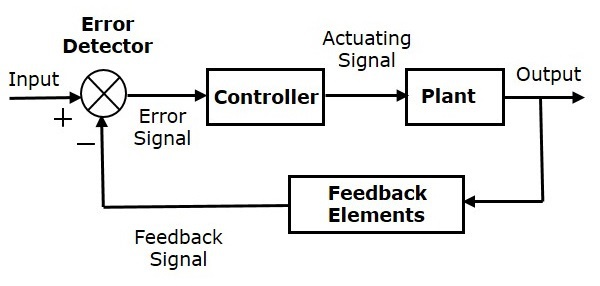
\includegraphics[scale=0.40]{images/closed_loop.jpg}
    \caption{Schematic diagram of a closed-loop control system. The feedback element which is used to correct the errors between the target output (which is a function of the input executed in ideal circumstances without noise and disturbances) and the observed output. The controllers are typically devices such as PLCs or microcontrollers running firmware.}
    \label{fig:control system}
\end{figure}


\begin{itemize}
    \item \textit{Controller:} Controller is a component that takes in the sensor values and converts it into control commands $z_k$ that is to be sent to the actuators. For example, the controller could be a PID controller that estimates and keeps track of position. We could have similar controller to provide feedback-based control to attitude(roll, pitch and yaw) of a UAV.
	\item \textit{Plant or Process:} The physical phenomena of interest, called the physical environment. For example, the position of a UAV or the acceleration of a UAV. The controller's task is to moderate the plant and steer it to the desired output. The controller accomplishes this using actuators. Actuators are components that executes the control commands sent by the controller. Typically, actuators are components such as motors and propellers that causes a change in physical environment around the CPS.
	\item \textit{Feedback Elements:} These are components which sense the outputs driven by the controllers and transmits it in a time-series, denoting the measurement of physical environment at every time instance. For example, the GPS sensor or accelerometer in a UAV is a sensor that sends in time series of position values to the controller.
 

\end{itemize}

\textbf{Cyber-Physical Systems(CPS)} CPS's are examples of closed loop systems, since, the physical subsystem executes commands from the computing system and the the computing subsystem consumes the sensor values perceived by the physical subsystem. Typically a physical subsystem consists of a combination of sensors and actuators. These two subsystems are connecting to form a feedback-based control system as shown in Figure \ref{fig:cps}

\begin{figure}
    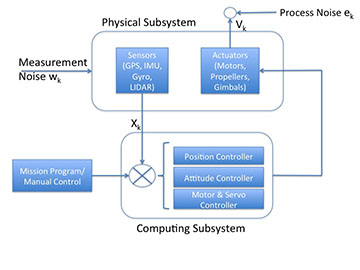
\includegraphics[scale=0.60]{images/cps-fig-small.jpg}
    \caption{Schematic diagram of a Cyber-Physical System, showing the Cyber and Physical realms in action. The diagram also shows the two kinds of noise in play in the physical world -- noise in measurement and noise in environment. These cause imperfect sensing and imperfect actuation repectively..}
    \label{fig:cps}
\end{figure}
%Insert picture of a cyber-physical system here with both cyber and physical aspects

As Figure \ref{fig:cps} describes, there are cyber and physical realms that are feedback control with one another. The mission control program could be as simple as preset waypoints on a map or it could be as complex as a neural network taking multiple inputs. In the case of a UAV, it could be something external such as manual commands using radio controller joystick to drive the UAV.  There are two kinds of noise that are in play here. First is the measurement noise, which gets mixed with the sensors while a measurement of the physical environment is obtained. In short, this noise accounts for imperfection in measurements and is typical in all measurement-based systems. Second is the process noise, which gets mixed with the environment when the controller drives the outputs to physical environment. In other words, this noise accounts for imperfect actuation.

\subsection{Attacks on CPS Systems}
There are multiple ways to compromise a CPS system. However, we would be generalizing the attacks into three broad categories. First, the attack could be on one of the actuators. This is typically done by intercepting the control command executed by the actuator to effect the physical environment around the CPS. In other words, the control command executed differs wildly from $v_k + e_k$ as it should be from Figure \ref{fig:cps}. This could result from the actuation mechanism itself being compromised or by accepting a control command from an untrusted agent. This false actuation will affect the measured variables of the physical environment and thereby the sensor measurements are also tampered.

Second, the attack could be on the sensors in the system. This is typically done by altering the perception of the physical environment around the CPS system. As a result, the sensor measurement used by the controller would be different from the real state of the measured variables. In other words, the physical process being measured differs wildly from $x_k + w_k$. Similar to attacks on actuators, attacks on sensors have the effect of circulating in the closed loop system, once injected.

Third, and perhaps the most grievous, is the case of the controller device getting compromised as well, giving the attacker unlimited control to implement any outcome. To detect this, one would need an unbiased view of the CPS system from an external vantage point that could be a trusted ground control station or a trusted UAV to perceive the state and compare it with the monitored UAV. 

In this paper, we are primarily concerned with attacks of the first two types of attacks -- attacks on actuators and sensors. We would be focusing on the design on a control-invariant framework that can help detect the attacks described. At a high level, our framework takes in measurements, say from sensors, $x_k$ and control commands, $V_k$  that are pushed out by the controller to the actuator and makes a binary decision of an attack via an anomaly detection technique. It is important to note that the idea of monitoring sensor measurements and control commands to identify issues with sensors, actuators or controllers is not a novel idea and is a popular idea in fault detection research. However, this style of fault detection relies on physical as well as spatial diversity (the technique of having multiple sensors or controllers and decide on majority voting) or functional redundancy(eg., measure a quantity directly as well as indirectly -- such as position being measured by double integrating acceleration). Furthermore, this sort of detection is not sufficient for an attacker, since, the effort to compromise multiple sensors having one compromised is O(1) -- via attack reuse. These attacks are shown in Fig \ref{fig:cps-attacks}. 

\begin{figure}
    \centering
    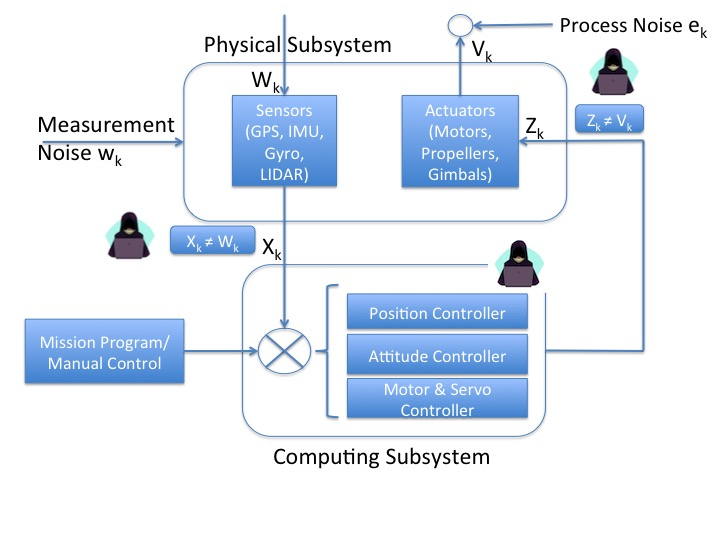
\includegraphics[scale=0.33]{images/cps-attacks.jpg}
    \caption{Attacks on a CPS system. The attacks can be on three regions -- sensors, actuators or the controller. The sensors and actuators form the physical subsystem and the controller which does the computing forms the compute subsystem of the CPS. In this paper, we are concerned only about the physical subsystem. The compute subsystem can be secured by using good security practices such as Control Flow Integrity \cite{abadi2005control}. }
    \label{fig:cps-attacks}
\end{figure}

\begin{figure*}
    \centering
    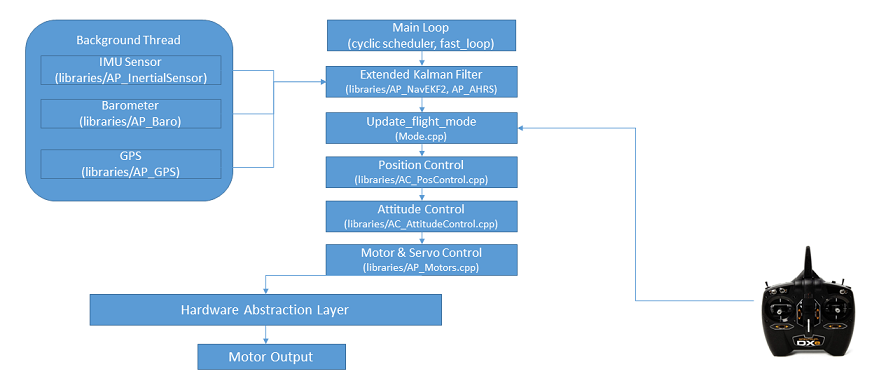
\includegraphics[width=\textwidth]{images/ardupilot-small.png}
    \caption{Architecture of an Autopilot. The main loop is run by a cyclic scheduler which polls sensor values periodically. The sensor values are fed into an Extended Kalman Filter which is used to estimate(correct) the sensor values and send it to position and attitute control layers. These are implemented as PID controllers which calculate the control signal that needs to be sent to the motors to perform the required navigation}
    \label{fig:ardupilot}
\end{figure*}

\subsection{Threat Model} The adversary is assumed to attack the physical components of the UAV viz., the sensors and/or actuators. The mode the adversary takes to accomplish this is irrelevant to our problem. Additionally, the adversary is assumed to not possess a knowledge of one of the following: 1) The Low-level parameters used in the controller, 2) The Physical model of the UAV. Lastly, we will assume that the UAV is not compromised via the computing subsystem and the compute subsystem is assumed to be secure.

\subsection{Software Architecture of a UAV System} UAVs need a navigation software to make it \textit{unmanned} as opposed to just receiving commands from a radio transceiver and navigate accordingly. This software performs the navigation by computation based on reading sensor values and  Ardupilot is an open-source autopilot software that is capable of controlling autonomous drones, helicopters, boats, submarines, and antenna trackers. The ardupilot software suite consists of navigation software, called firmware when it is compiled into a binary for microcontroller-based hardware hosts \cite{anderson2016ardupilot, wiki:xxx}.

As seen in the Figure \ref{fig:ardupilot}, Ardupilot software stack consists of a cyclic scheduler that triggers a main loop at periodic intervals. The main loop consists of a polling of GPS and IMU sensors which give the position and attitude of the UAV. The GPS sensors give an estimate of the linear position by means of latitude and longitude values. The IMU is a unit consisting of accelerometer, gyroscope, and magnetometer. Typically, there is one accelerometer,gyroscope and magnetometer per axis for each of the three vehicle axes: pitch, roll and yaw. The three vehicle axes are shown in Figure \ref{fig:imu}. It is shown in CPS and optimal control theory research \cite{dissanayake2001solution} that using these sensors in isolation leads to drift and estimation errors. As a result, these values are passed onto an Extended Kalman Filter(EKF) which is used to correct these errors and provide \textit{optimal estimation} for sensors in the presence of noise. Let us consider the example of position and attitude estimate, which is the problem of estimating the coordinates of x, y and z along with their angular versions (roll, pitch and yaw). EKF achieves this by fusing the values from IMU and GPS in conjunction with its knowledge of estimated noise in each of the measurement channels. Note that this approach of correcting sensory measurements can equally be applied for other sensors such as barometer (pressure) or wind sensor as well though those are less interesting from a security standpoint \cite{raginskyuiuc}.

\subsubsection{The Extended Kalman Filter} The following steps are a highly non-mathematical gist of how the Extended Kalman Filter(EKF) works in practice:

\begin{enumerate}
    \item IMU angular acceleration values are double integrated to derive angular position values
    \item The IMU angular position vales are converted from the frame of the UAV to the frame of earth. Using this, a corrected value of IMU angular acceleration value is calculated.
        \begin{itemize}
            \item This is done since GPS values are along the earth's coordinate system but IMU values are along the UAV's roll, pitch, yaw coordinate system. 
        \end{itemize}
        
    \item The corrected IMU accelerations are single integrated to derive velocity estimates
    \item The IMU velocity estimates are single integrated to derive position estimates.

\noindent Steps 1 to 4 collectively is known as the  \textit{State Prediction} process. State is a variable that is to be estimated such as roll, pitch, yaw.
    
    \item The IMU keeps an estimate of accelerometer noise. This is used to estimate the growth in errors in position, velocity and their angular counterparts. These errors are captured in a large matrix called the \textit{State Covariance Matrix}.
    
\noindent Note that until now, GPS values are not used. Now suppose a GPS measurement comes in.

    \item The GPS measurement is used to calculate the difference between position calculated in Step 4 and the GPS measurement. This value is called \textit{innovation}
    
    \item The innovation value, state covariance matrix is combined with the GPS noise estimate (similar to the IMU accelerometer noise) to obtain a correction in position, velocity and their angular counterparts.
    
    \item The state covariance matrix used in step 5 is updated and the process is repeated.

\end{enumerate}
 
\subsubsection{The SLAM problem} Simultaneous Localization and Mapping, better known as SLAM, is an algorithms used in robotics. This is common when a UAV enters a hitherto unknown environment having  to perform spatial exploration and navigate accordingly. The SLAM problem is solved by using a Extended Kalman Filter, which has the capability to optimally estimate the state of a UAV in presence of noise. Again keeping the discussion highly non-mathematical, SLAM solution consists of 3 operations, iterated at every single time-step: \cite{bailey2006consistency}

\begin{enumerate}
    \item The UAV moves, reaching a new point of the scene. Due to unavoidable noise and errors, this motion increases the uncertainty in the position values of the UAV.
    
    \item The UAV discovers interesting features in the environment, which need to be incorporation into the map. This step is called Mapping and the features are called landmarks. Due to errors in the sensors, the location of these landmarks is uncertain. This is in conjunction with the uncertainty in the position values of the UAV. Thus, there are 2 uncertainties at this stage.
    
    \item The UAV observes landmarks that has been previously mapped. This is used to correct the position of landmarks and the UAV's position. Thus, after this step, the position uncertainty of the UAV and position uncertainty of the landmark are corrected.
\end{enumerate}

These values obtained in this three steps are fed into an Extended Kalman Filter(EKF) to correct the errors and build an automated solution for navigation.


\section{Experiments}


\section{Conclusions}


\appendix

%\section{Location}

%Note that in the new ACM style, the Appendices come before the References.

%\section{Related Work}
The idea of using models to characterize normal behavior has been tried across a wide spectrum of systems ranging from industrial control plants \cite{wang2014srid}, capturing the physics of sensors \cite{shoukry2015pycra}, medical devices \cite{hei2013pipac}, and other control systems \cite{mclaughlin2013cps}. The equivalent of a model in control theory is called \textit{state estimation}. The central idea is to characterize the variations in key parameters as well as the noise that is inherent in the physical environment and the measurement. Models typically capture a universal law in the domain of application. For instance, in industrial control plants, laws of fluid dynamics such as Bernoulli's equations can be used to capture the model. However, as the applications of models have varied wildly from one another, there has not been enough discussion to provoke the use of model-based anomaly detection in a general sense. \\

\subsection{Security \& Privacy in CPS} Security and privacy of CPS systems is a well-researched area. An example is is verification of control code by an embedded system before it reaches the Programmable Logic Controller(PLC), Remote Terminal Unit or Intelligent Electronic Device(IED) \cite{mclaughlin2014trusted}. This work came out in the context of the popular Stuxnet \cite{falliere2011w32} security breach and triggered a bunch of other works in this space. Examples being security of embedded devices \cite{lemay2009cumulative}, the automatic generation of malicious PLC payloads \cite{mclaughlin2012sabot}, medical device security \cite{rushanan2014sok}, vulnerability analysis of vehicles \cite{checkoway2011comprehensive}, and of automated meter readings \cite{rouf2012neighborhood}. There is work on CPS privacy such as smart grids \cite{jawurek2012sok}, vehicular location monitoring \cite{hoh2008virtual}, and location privacy \cite{shokri2011quantifying}. These are related but complementary to the problem that we are describing in this paper. 

Instead, in this work,we are going to be focusing on using measurements of the physical world via sensors to build up an indicator of attacks. This work is inspired by the work on false sensor measurements \cite{liu2011false}, or false control signals such as manipulating vehicle platoons \cite{gerdes2013cps}, manipulating demand-response systems \cite{tan2013impact}. The question we ask is this: \textit{How do we raise a flag when something is wrong with sensors or actuators?}. Intrusion detection is a problem that is closely related to this. A classic paper which considers intrusion detection in industrial control networks is Cheung et al. \cite{cheung2007using}. It is noted in this paper that the technique of network anomaly detection is more effective in bounded, finite control networks where network flows are more regular and stable compared to the traditional computer networks used in the internet.

\subsubsection{Secure System Identification} One of the main areas of research in the CPS community is to find efficiently the subset of sensors that are sending false information \cite{chong2015observability}. These systems are assumed to satisfy the equations for Linear, Time-invariant systems which has been noted earlier. The main idea here is to solve a combinatorial optimization problem to find a subset of sensors, which are assumed to be safe, to generate adequate state estimations. Shoukry et. al \cite{shoukry2018smt} proposed a search algorithm based on Satisfiability Modulo Theory(SMT) to speed up the search of possible sensor sets and extended this to systems subject to random noise \cite{mishra2017secure}. In particular, it was noted that the number of sensors used to monitor the process has to be atleast twice the number of sensors under attack. In this paper, the authors  assume that the controllers and actuators can be trusted. Furthermore, there is a degree of hardware redundancy assumed in this paper which might not be always true in practical systems

\subsection{Attacks on UAVs} Attacks on UAVs do not surprise anymore. In \cite{checkoway2011comprehensive, koscher2010experimental}, the internal vehicular networks are infiltrated by subverting the CAN bus. CAN bus, being a broadcast-based protocol is shown to be subverted by an adversary with a laptop having a wireless card. In \cite{ishtiaq2010security}, the authors exploit a car tire pressure sensing system, which uses RF wireless motes. Kerns et. al \cite{kerns2014unmanned} consider how the Global Positioning System (GPS) signals can be used to take over UAVs. The attacker generates a counterfeit GPS signal and sends it to the GPS antenna of the UAV. This replaces the real GPS reading with a fake reading. The paper also proposes a detection strategy by modeling the UAV's state and using a \textit{residual test} (a system that takes in sensor readings outputs a signal called the residual as per a mathematical formulation). This paper is interesting and shows 2 attacks -- one where the attacker is detected, and another where the attacker manages to keep all the residuals below the threshold while still steering the aircraft to their location. Optical sensor input spoofing \cite{davidson2016controlling} involves obtaining an implicit control channel by tricking optical flow sensors with a fake ground plane. In \cite{son2015rocking}, the authors propose using a gyroscopic sensor attack with intentional acoustic noise to crash drones. Furthermore, the authors of \cite{trippel2017walnut} compromise accelerometers by injecting acoustic noise in a more controlled manner, as a more advanced form of attack. Anti-lock Braking System(ABS) attack \cite{shoukry2013non} involves injecting magnetic field to spoof the wheel speed sensor. In \cite{highnam2016uncrewed}, an attacker with an antenna and malicious ground station can compromise a benign UAV by sending malicious packets. In \cite{petit2015remote}, there are attacks on camera-based ground vehicles by relaying and spoofing signals.


\subsubsection{Detecting Attacks on UAVs} Detecting attacks on UAVs has been explored by multiple angles. The approaches tried out by the community can be classified into four buckets. Note that all of these approaches can be broadly called as \textit{Model-based} approaches.

\begin{enumerate}
	\item Signature-based detection
	\item Machine Learning (Classification)
	\item System redundancy
	\item Formal specification
\end{enumerate} 
 
Signature-based detection consists of a monitoring mechanism and compares it with pre-determined attack patterns known as attack signatures. This approach is popular among anti-virus corporations as well and relies on maintaining a database of signatures, which might curtail the usefulness of this approach. Machine learning-based approach monitors abnormal behaviors using a technique such as trained neural network or deep learning. The normal behavior is defined by supervised and unsupervised methods in the training phase. The disadvantage of this approach is the large training dataset that is needed to cover all the corner cases. Although unsupervised learning systems remove the need for labeled data, the issue of high false positives remain. Redundancy-based techniques duplicate key system components (such as the controller) and cross-check their states/outputs at runtime to detect intrusions/attacks/anomalies. The redundancy can be in hardware or it can be in software or a combination of both. However, from an attacker's standpoint, having redundant sensors increases the attack surface while increasing the attackers effort by only a constant effort. In effect, this seems like the wrong game to play with the attackers. Formal specification based attacks rely on program execution invariants to capture normal system operations. The end result is a state machine that can be used to detect anomalous program states and transitions to detect anomalies/attacks. A summary of attack detection methods used in UAVs is given in Table \ref{table:attack-detection-uav}.

\begin{table}[h]
\caption{Some attack detection techniques used in UAVs. There are four broad techniques used for detecting attacks on UAVs and other CPS-based systems.}
\begin{tabular}{ |p{3cm}|p{3cm}|}
 \hline
 \multicolumn{2}{|c|}{Attack Detection Methods used in UAVs} \\
 \hline
 Type of Strategy used & References \\
 \hline
 Signatures & \cite{gao2014cyber, kaur2013automatic}\\
 \hline
 Machine learning & \cite{abbaspour2016detection, chen2018learning, junejo2016behaviour, shen2014novel}\\
 \hline
 System redundancy& \cite{fei2018cross, frank1990fault, xu1987fuzzy, yoon2017virtualdrone}  \\
 \hline
 Formal specification & \cite{bak2011sandboxing, mitchell2014adaptive,  mitchell2015behavior, zimmer2010time}  \\
 \hline
\end{tabular}

\label{table:attack-detection-uav}
\end{table}






%\begin{acks}
% TODO: For the submission, don't include acknowledgments since they would most likely deanonymize you.
%\end{acks}
 % TODO: replace with your brilliant paper!

\bibliographystyle{ACM-Reference-Format}
\bibliography{ccs-sample}

\end{document}
